\subsection{Product perspective}

\subsubsection{Scenarios}

\subsubsection*{User wants to register with an account to BBP}
A user U wants to join the BBP community. U downloads the app from their favorite AppStore and opens it. U then goes to the registration page, enters their data (Username, Email, Password) and proceeds to the authentication phase. A message is sent to their email address and U must confirm their account. After that, they are ready to log in

\subsubsection*{Registered User wants to log in with their account to BBP}
A registered user RU wants to log into their BBP account. RU opens the application on their smartphone and goes to the Login Page. Here, RU inserts their Username and their Password. BBP will hash the password and try to match the fingerprint with the one associated to RU account. If it is correct, the login process ends. If not, an error message appears and another attempt at login can be done.

\subsubsection*{Registered user enables automated mode}
A registered user RU logs into the BBP application and enables the automated mode in the home page. The application prompts RU into authorizing access to the device's sensors (GPS, accelerometer, and gyroscope) as well as background execution to allow the system to start collecting data from their mobile device. The application then starts monitoring things like speed, vibrations, among other data to determine whether the user is riding a bike or not.

\subsubsection*{Registered user disables automated mode}
A registered user RU disables automated mode. After this action, BBP no longer collects location or sensor data automatically. Future paths must be recorded manually if the user wants to add new ones. The user can re-enable automated mode at any time.

\subsubsection*{Registered user does a bike ride with automated mode}
A registered user RU starts cycling with automated mode enabled. BBP detects the user’s speed and movement, confirming that the user is biking. During the ride, the system collects GPS coordinates and motion sensor data to reconstruct the path and identify possible obstacles. After the sensors detect that RU stopped cycling, BBP starts processing the just collected data and notifies RU (with a pop-up notification on their phone) that the path has been recorded and that needs revision to be published. RU can decide either to review the entry, or to ignore it and delete it.


\subsubsection*{Registered user wants to publish a path recorded in automated mode}
After their cycling activity, a registered user RU wants to publish the recently recorded path, and make it available for every other user. In doing this, they either press the pop-up notification or open the application by pressing the icon. BBP shows them a summary of the path, including detected issues. RU reviews the information, and changes the incorrect or problematic parts (if any). Finally, RU can publish the entry to the application, ready to be used by BBP.

\subsubsection*{Registered user publishes a bike path in manual mode}

A registered user RU accesses the manual entry section in BBP to add a new bike path. RU specifies the streets that compose the path and assigns a status to each road that composes the path. The user adds details like the presence of obstacles and surface type. Once the information is complete and reviewed, RU publishes the path, allowing it to become visible to all the user base.

\subsubsection*{Registered user records a trip}
A registered user RU begins recording a new cycling session using the BBP application. If the access of the sensors (GPS, accelerometer, and gyroscope) and background execution has not been granted yet, the application will prompt the user to allow access. BBP records the trip details through the device's sensors, including: start and end timestamps, total distance covered, and average speed. Upon completion, RU can save the trip to their personal log and view statistics. 
Asynchronously, once the trip is finished, BBP will use a external service that provides weather data to enrich the trip's data with information such as: Temperature, wind speed, and precipitation.

\subsubsection*{User searches for paths}

A user U, whether registered or not, specifies an origin O and destination D. BBP calculates, using the road stored in its database, all the possible bike paths between O and D. If multiple options are available, BBP displays them ranked by their path score, which depends on path status (calculated as a mean of all the statuses of the single roads in the path) and effectiveness. U can visualize the suggested routes on the map and explore details about obstacles and path condition.

\pagebreak
\subsubsection{Domain Class Diagrams} 

\begin{figure}[H]
\centering
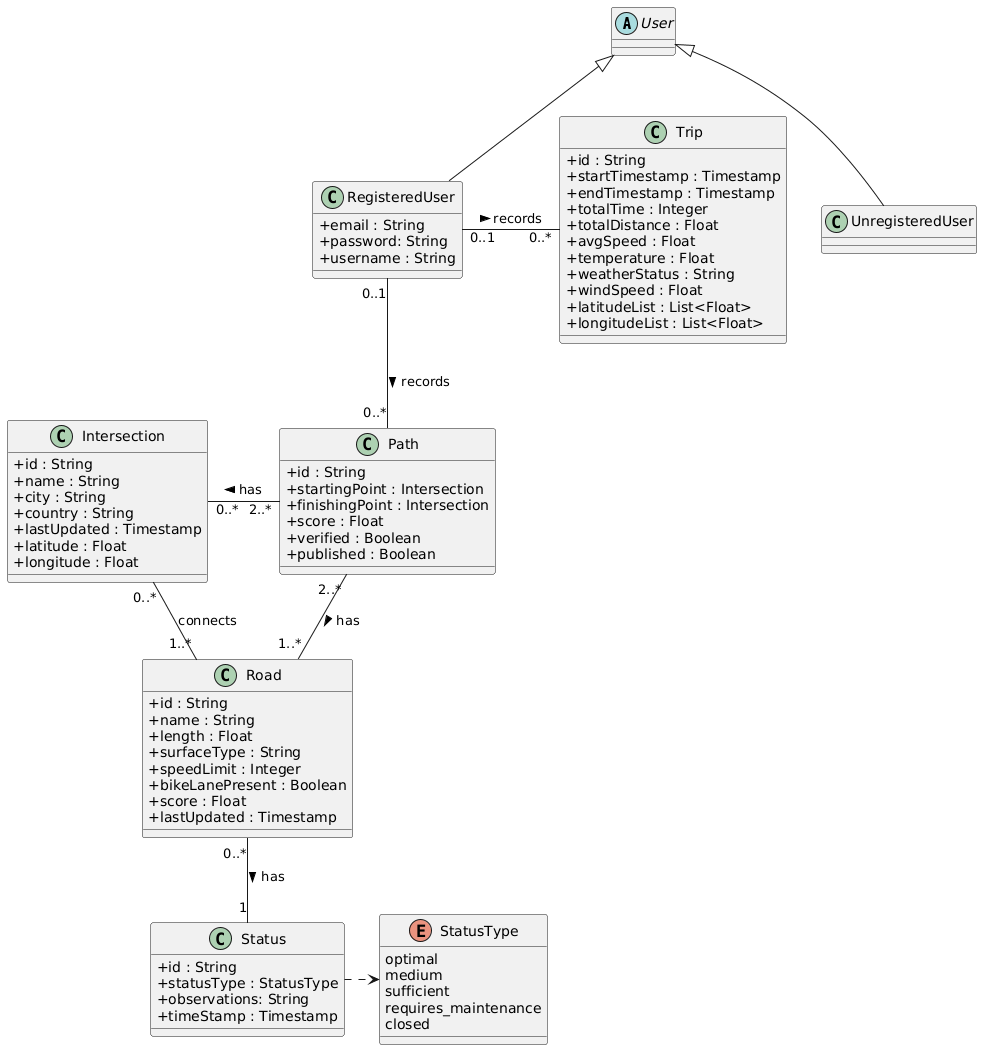
\includegraphics[width=\textwidth]{RASD/Images/Diagrams/Domain/domain-class-3.png}
\caption{\label{fig:domainclass}Domain class diagram for BBP.}
\end{figure}

This Domain Class Diagram ~\cite{uml_diagrams_class_2025} represents the entities involved in the domain of our system and
the relationships between them. Some important points to note:

\begin{itemize}[label=-]
    \item The system distinguishes between registered and unregistered users, with registered users capable of recording trips, contributing data, and making information publishable, while unregistered users can only access information but not contribute or personalize their data.
    \item Registered users can record trips, which include detailed statistics like total time, total distance, average speed, and meteorological data (weather, temperature, wind speed) when available, supporting richer activity logging. 
    \item Paths connect intersections (nodes), utilizing roads as their links, mirroring the real-world and supporting route computation for origin-destination queries. Each path can be marked as verified, published, and scored, facilitating ranking and quality assessment based on both user input and system-calculated factors. Roads and their status types (e.g., optimal, requires maintenance, etc.) allow precise condition reporting, which is crucial for route planning and safety.
    \item The system allows both manual and automated data entry for path and obstacle information, supporting flexibility for user input and leveraging sensor data for finer granularity. Automated mode requires post-capture user verification, addressing the problem of false positives (e.g., erroneous pothole detections), ensuring data quality before publication.
    \item The system supports community-driven data integration, where multiple user contributions about the same path or road are aggregated, prioritizing information based on freshness and majority consensus for better accuracy and reliability. 
    \item Both registered and unregistered users can visualize computed paths based on road status and path effectiveness , helping users choose optimal routes.
\end{itemize}

\newpage

\subsubsection{State Machine Diagrams}~\cite{STM}
\textbf{The registered user records a Trip}
\begin{figure}[H]
    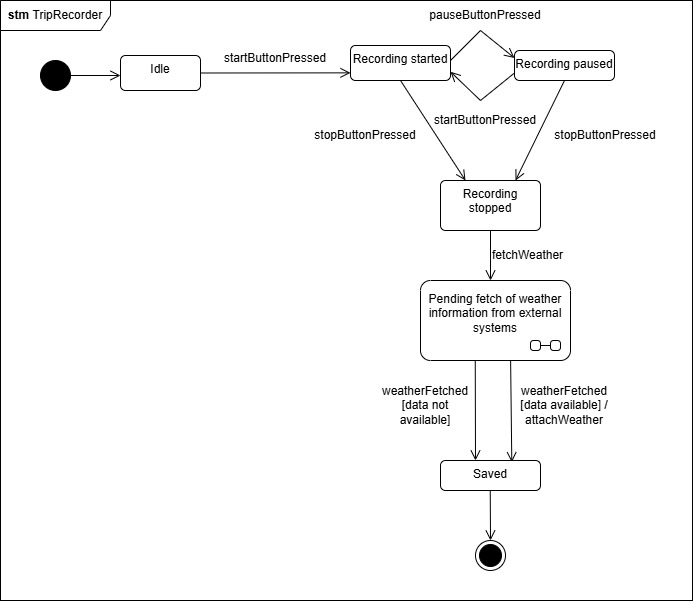
\includegraphics[width=\textwidth]{Images/Diagrams/State Machine/TripRecordingSTM.jpg}
\end{figure}
This state machine describes the different states in which the TripRecorder can be found. At first, the machine is in idle state, waiting for the user to decide if they want to start a recording.\newline
After pressing the start button, the application starts recording, acquiring information on the streets and intersections crossed by the biker, their average speed, max speed, time passed and distance traveled. The user can decide, at any time, to pause and resume the recording while cycling.\newline
At the end of the entire trip, the stop button is pressed and the data is processed.\newline
During data processing, the application asks an external weather reporter system additional data, to enrich trip details. If this information is present, they are attached to the trip recording.\newline
Regardless of the outcome, the trip is saved and now ready to be reviewed.\newline
\newpage

\textbf{The registered user records a Path}
\begin{figure}[H]
    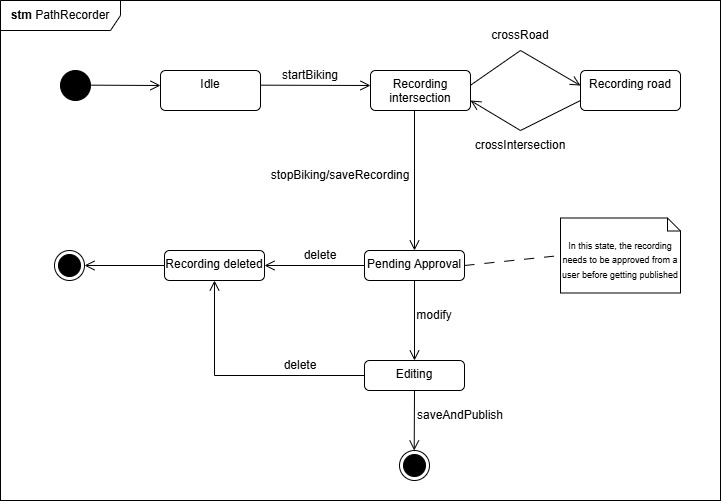
\includegraphics[width=\textwidth]{Images/Diagrams/State Machine/PathRecordingSTM.jpg}
\end{figure}
This state machine describes the different states in which the PathRecorder can be found. Please note that this diagram is showing the \textbf{Automated Mode} only. The \textbf{Manual Mode} is very similar, and journaling is delegated to the user.\newline
After selecting the automated mode in the home page, the machine goes in idle state, waiting for the user to start biking.\newline
When the external sensors (GPS, gyroscope, accelerometer) detect a possible cycling motion, the application starts recording the cycling activity. At this point, roads and intersections information are acquired using the same sensors (especially estimating road conditions and position into the map) until the biker stops cycling.\newline
All the collected data is then saved and ready to be reviewed. Considering the possibility of having false positives, the path must be reviewed by the user before it reaches the published state. In any moment of this process, the path can be discarded and never published.\newline
At the end of the editing phase, the path is saved and published, now available to be used by the application to find paths for other users.
\newpage
\textbf{User searches for Paths}
\begin{figure}[H]
    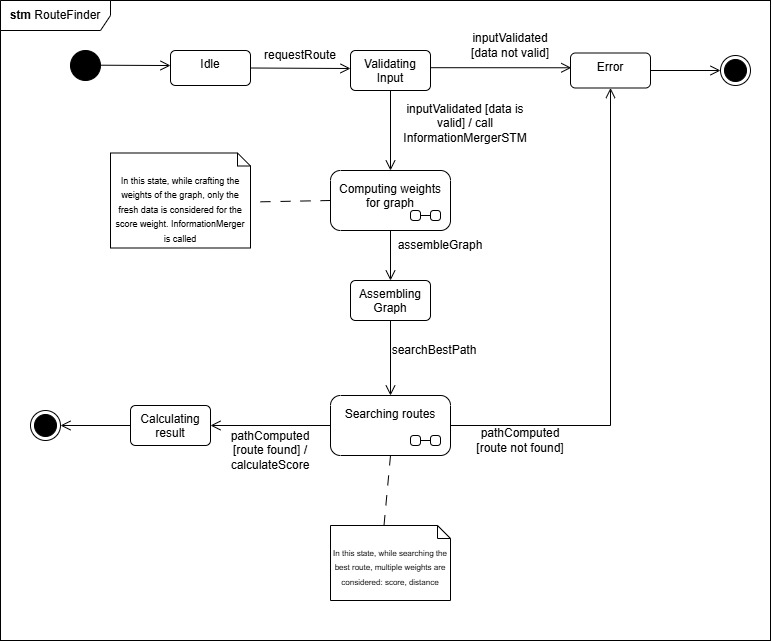
\includegraphics[width=\textwidth]{Images/Diagrams/State Machine/RouteFinderSTM.jpg}
\end{figure}

This state machine describes the different states in which the RouteFinder can be found. This machine is used to calculate the possible routes between a starting point and an ending point selected by the user.\newline
After inserting the start and ending positions, a request to the machine is sent and the input validated. An error occurs if the positions do not exist inside BBP.\newline
The chosen model to represent this problem is a graph, with intersections as nodes and roads as weighted arcs. Please note that, if the starting point is not an intersection but positioned inside the road, an additional parameter is multiplied to the weights to express the real position inside the graph. These weights need to be retrieved from BBP database. In particular, the roads "conditions" could be ambiguous due to multiple entries added at the same time. To solve this issue, the condition weight is calculated by another machine (see  ~\hyperref[fig:informationmerger]{InformationMergerSTM} below) to evaluate the real current condition of the road.\newline
The graph is then built and routes found by using classical route searching algorithms in graphs. For each route, a score is calculated to be correctly displayed in the mobile application.
\newpage

\textbf{The road score is calculated}
\begin{figure}[H]
    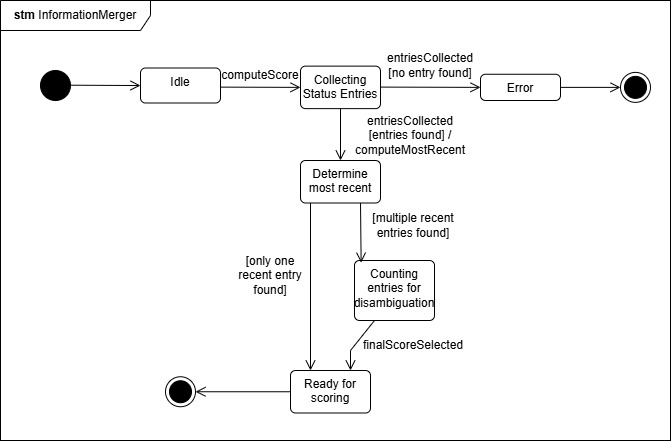
\includegraphics[width=\textwidth]{Images/Diagrams/State Machine/InformationMergerSTM.jpg}
    \label{fig:informationmerger}
\end{figure}

This state machine describes the different state in which the InformationMerger can be found. This machine is used to merge and present the current and most fresh information to the user.\newline
When it is asked to compute a specific road condition, the machine fetches the status entries from the application database regarding that specific road and uses the "timestamp" attribute to determine the most recent entry.\newline
To consider also the possibility of multiple entries with the same timestamp, if the machine finds this "ambiguity", it also performs a "disambiguation" operation: it counts, for every different label of the road condition, the entries with the same timestamp and returns only the one with the biggest cardinality. If even in this case, it's present an ambiguity, it returns the worst label of the group (this guarantees the safety of the biker, avoiding any possible injury).

\subsection{Product functions}

\subsubsection*{Sign Up}

Users can create a new account by providing the necessary personal information to register with the Best Bike Paths (BBP) system. The required personal information includes:
\begin{enumerate}
    \item Username
    \item Email
    \item Password
\end{enumerate}
After submitting the registration form, a confirmation email will be sent to the user's email address. Once the user confirms their account, they will be considered successfully registered and will be redirected to the login page to perform their first login.

\subsubsection*{Login}
The BBP application allows users to sign in using an email address and a password. After inserting the credentials, BBP will check the correctness of the information (f.e. that an email address is associated to an account, or that the account has been successfully verified) and will redirect the user to the home page if that is the case.
If an error during this step has occurred, BBP will notify the user about it.

\subsubsection*{Record a trip}
Registered users can record their cycling activities using the BBP application. When a user starts trip recording, the system collects data from GPS, accelerometers, and gyroscopes to accurately track the route and motion. Upon trip completion, BBP processes the collected data to calculate various statistics, including total distance covered, average speed, and total time spent. The recorded trip is then saved to the user's account and can be viewed through the application interface.

\subsubsection*{Enrich a trip's data}

Once a trip is uploaded to BBP, an asynchronous process begins to enrich the trip data with meteorological information such as weather conditions, temperature, and wind speed. This data is retrieved from an external service and then integrated into the existing trip record. After the trip is updated, users can view the additional meteorological details on the trip detail interface.


\subsubsection*{Insert and publish a bike path}

The BBP application offers two modes for collecting raw data, depending on the user’s preference.\\
\begin{enumerate}
    \item \textbf{Automated Mode}\\
In the automated mode, the BBP application leverages all the built-in sensors of the user’s device to automatically gather the necessary raw data for reconstructing the complete path. Specifically, the GPS sensor is used to track the user’s journey, while motion sensors such as the gyroscope and accelerometer help assess the difficulty of the path at each point—enabling the detection of potholes or other irregularities affecting the ride quality.
To improve the reliability of the collected data, users are encouraged to review and confirm the system’s detections once the journey is completed.
    \item \textbf{Manual Mode} \\
The manual mode is simpler and entirely relies on the user’s honesty and accuracy when entering information. In this case, the user must manually specify the names of the streets included in the path and indicate their respective conditions. If the condition of a path is not "Optimal", the user can also add details about the problems encountered.
\end{enumerate}

\subsubsection*{Browse bike paths}

Any user can explore available bike paths by specifying origin and destination points. The system displays the routes on a map, presenting relevant information such as path conditions, obstacles, and maintenance status to assist in route selection. When multiple paths are available, BBP visualizes them and assigns a score to each, reflecting the quality of the path based on its effectiveness and current condition. This scoring helps users evaluate and choose the most suitable route for their needs.

\subsubsection*{Score a path}

The BBP system collects information from multiple paths and visualizes it through a scoring mechanism. The score is primarily based on the condition of the path and its effectiveness in enabling the user to reach the desired destination from a given origin. The score is given by the user using tags.

\subsubsection*{Merging of similar paths and updating statuses}

When multiple users provide information about the same bike path, BBP merges the data by evaluating the recency of each input and the number of confirming reports. This merging process automatically updates the path’s status to reflect the most accurate, consensus-driven information. Users may tag paths with statuses such as “Optimal” or “Requiring maintenance.” During data consolidation, BBP prioritizes the tag from the most recent input to ensure the path status remains up to date.


\subsection{Users characteristics}

Any user — whether an experienced rider or completely new to biking — can join the platform through the application. Each path shared by a user remains anonymous and is not linked to its creator. As a result, all related paths are automatically collected and anonymously made available to other users. The user is able to insert information, scores of hardness, and any kind of information to any path taken. Furthermore, the user can even relies on the platform to automatically generate the information, however, a final check to the information must be provided. Every user profile and information are private and remain hidden from other users.

\subsubsection{Any user (non-registered and registered users)}

All users, whether registered or not, can explore the information provided by Best Bike Paths (BBP). They can use the map interface to enter an origin and a destination, asking BBP to show possible bike routes between those points. When several options exist, the system ranks them by a score based on path condition, safety, and route effectiveness. \\
Users can view each path’s detailed information, including maintenance status, surface quality, and possible obstacles like potholes. However, unregistered users cannot record trips or add new information, but still access BBP’s main navigation and route-finding tools supported by community data.

\subsubsection{Registered users}

Registered users gain access to extended features supporting individualized interaction and community contribution. They may record personal cycling activities, which are stored within their user profiles and supplemented by metrics such as total distance traveled, average speed, and detailed trip analytics. BBP may augment recorded trips with meteorological data, including weather conditions and temperature, sourced from external services. \\
Furthermore, registered users can contribute path information via two mechanisms: manual and automated. Manual mode allows users to annotate routes with names and assign path statuses. Automated mode enables BBP to collect and analyze path data in real time using mobile device sensors, subsequently allowing users to confirm or revise detected obstacles prior to publication. Validated contributions may be made publishable, with BBP consolidating multiple reports to reflect the most current and consistent community knowledge. These functionalities ensure that registered users can both improve and benefit from the evolving quality of information within the platform.

\subsection{Assumptions, dependencies and constraints}

\subsubsection{Regulatory policies}

The application is designed to enhance the overall user experience by providing an intuitive and efficient interface for data collection and sharing paths. Any user, regardless of their level of experience, can contribute to the platform by recording and publishing biking paths through the application. All related paths are automatically gathered and processed without any association with their original creator, ensuring that personal information remains strictly confidential. This approach guaranties full compliance with the General Data Protection Regulation (GDPR) \cite{gdpr_info_2025} and establishes a secure environment in which users can freely share useful data while maintaining anonymity. Furthermore, personal data are used exclusively for authentication and registration purposes — specifically for log-in via email, account setup, and authorization to access device sensors or third-party services. No personal information is used for any other purpose.

\subsubsection{Domain Assumptions}

\begin{itemize}
    \item \textbf{D1}: Each user rides a bicycle while the application runs in background in case of automated mode.
    \item \textbf{D2}: The internet connection remains relatively stable throughout the session.
    \item \textbf{D3}: Users are willing to review and refine the automatically collected information gathered by the device in the automated-mode.
    \item \textbf{D4}: Users are expected to provide accurate and non-misleading information when creating new paths.
    \item \textbf{D5}: Users do not use the application or the platform for purposes unrelated to biking activities or the exploration of new routes as a recreational activity.
    \item \textbf{D6}: Third-parties services provide reliable information to the application.
    \item \textbf{D7}: Hardware devices must provide reliable sensor data to the system to let it acquire the right performance data.
    \item \textbf{D8}: The date related to the new inserted path is correct.
    \item \textbf{D9}: The app is used where bike track already exists.
    \item \textbf{D10}: The biking paths have little to no cars presence.
    \item \textbf{D11}: The biking paths have speed limits compatible with the average speed of a bike.
    \item \textbf{D12}: Users will stop cycling when they want to end the recording of the path.
    \item \textbf{D13}: Users will give non-misleading information about their identity.
\end{itemize}

%Here is the command to refer to another element (section, figure, table, ...) in the document: \emph{As discussed in Section~\ref{sect:overview} and as shown in Figure~\ref{fig:metamodel}, ...}. Here is how to introduce a bibliographic citation~\cite{DAM}. Bibliographic references should be included in a \texttt{.bib} file. %

%Table generation is a bit complicated in Latex. You will soon become proficient, but to start you can rely on tools or external services. See for instance this \href{https://www.tablesgenerator.com}{https://www.tablesgenerator.com}.%


